\section{Modelling relevant aspects in EA}
\genHeader

The first step is to load an existing metamodel into EA. A complete and automatic import of existing Ecore files in EA is currently not possible and therefore,
\emph{relevant parts} of the existing metamodel (\texttt{GenModel}) have to be modelled manually. Although this might sound frightening (especially for
large, complex metamodels), the emphasis here on \emph{relevant} indicates that only elements that are needed for the transformation have to be present in
EA, where more can be added iteratively as the transformation grows. 

If you find this section challenging or unclear, refer to Part II: Ecore for a detailed review of metamodel construction.

\begin{stepbystep}

\item Open Eclipse and create a new metamodel project named \texttt{Ecore\-To\-Gen\-Model}, do not select the \texttt{Add Demo Specification}
option in the project wizard window.

\item A new specifications folder with the project name should have been loaded into the workspace.

\item Double-click the generated \texttt{Ecore\-To\-Gen\-Model.eap} file to open your project in EA. 
Explore the project browser and make note of the packages already present in EA under \texttt{eMoflon Languages}, especially \texttt{Ecore} which we shall use in this transformation.

\item Select the root note \texttt{My Working Set} and create a new package named \texttt{Gen\-Model\-Language}. 

\item Add a new Ecore diagram and model the elements as depicted in \Cref{fig_gMM}. You'll need to create the three EClasses on
the left, but \texttt{Ecore::EPackage} and \texttt{Ecore::EClass} are to be drag-and-dropped and pasted as links from the project browser. 

\vspace{0.5cm}

\begin{figure}[htbp]
\begin{center}  
	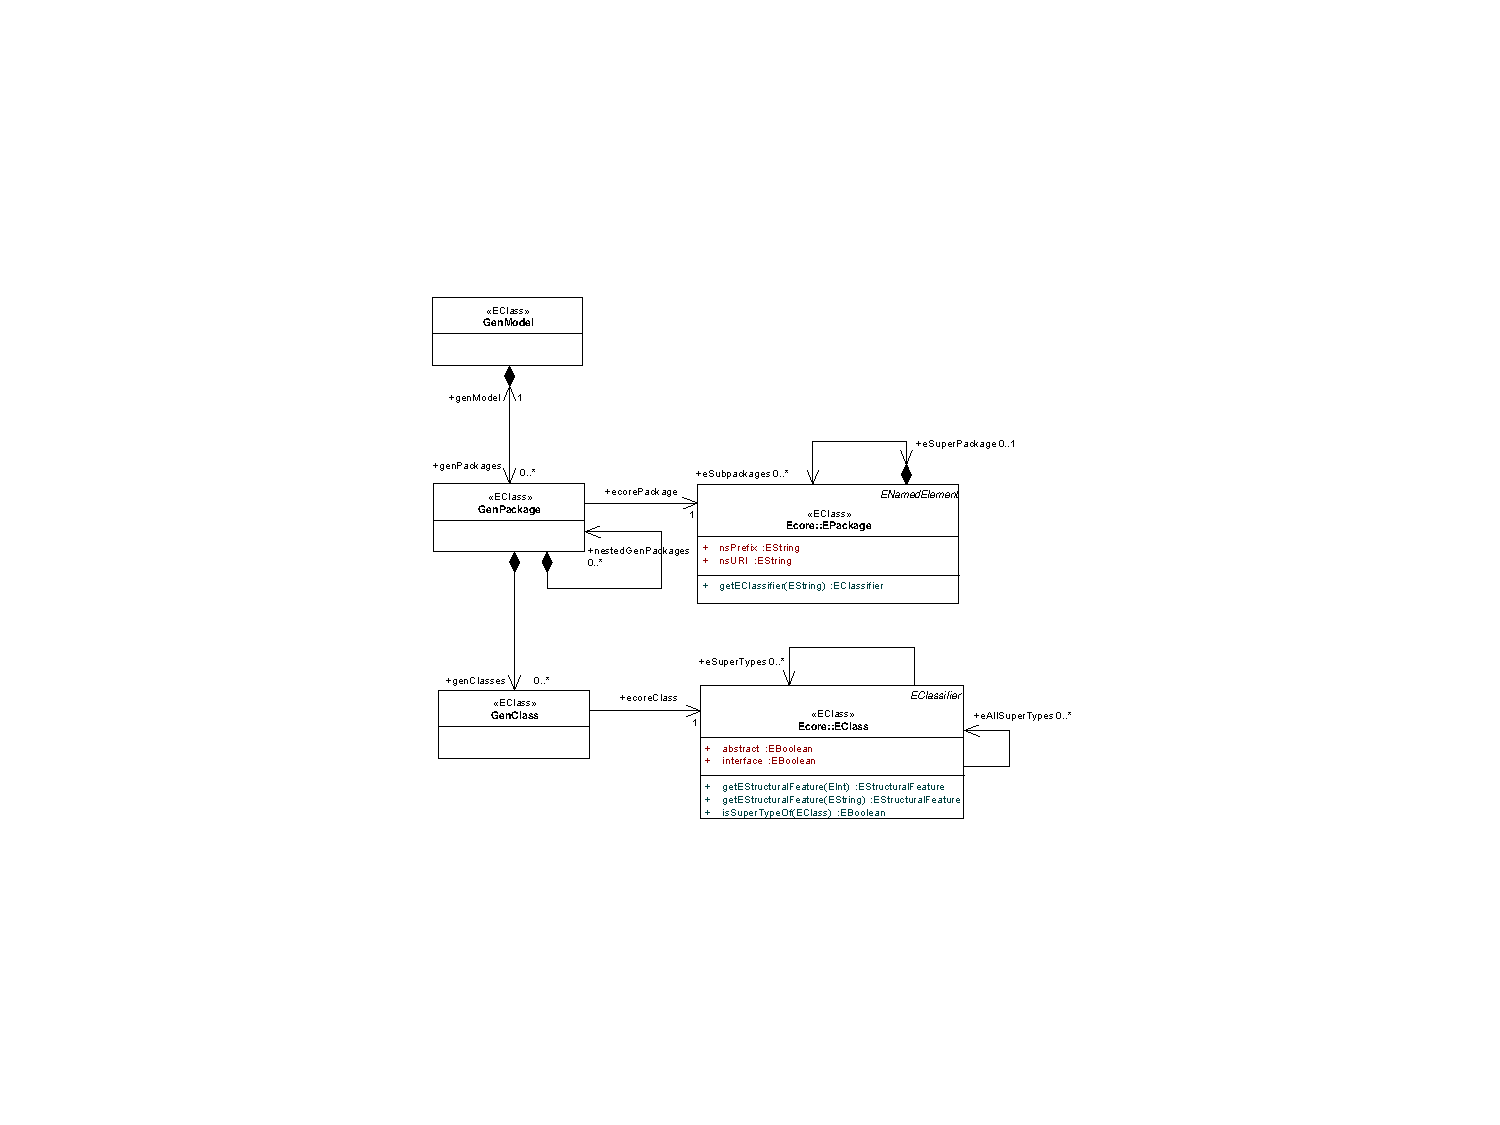
\includegraphics[width=\textwidth]{../../org.moflon.doc.handbook.05_miscellaneous/3_existingEMF/emfImages/CDGenmodel.pdf}
	\caption{Metamodel of \texttt{GenModel}}  
\label{fig_gMM}
\end{center}
\end{figure} 

\vspace{0.5cm}

\item Please note that the actual \texttt{GenModel} metamodel contains many more elements, but this subset is sufficient for our
task.
Although this subset can be incomplete, it must be correct and not contradict the actual \texttt{GenModel} metamodel in any way!

\item Navigate to the project browser again and create another package named \texttt{Ecore2GenModel}.  
This will contain the \texttt{Transformer} class; Create and complete its Ecore diagram as depicted in \Cref{fig_e2gm}.

\item Carefully double-click each method to create and implement their SDMs as depicted in \Cref{fig_pack2g,fig_transf}.
\end{stepbystep}

\newpage

\vspace*{2cm}

\begin{figure}[htbp]
	\begin{center}  
	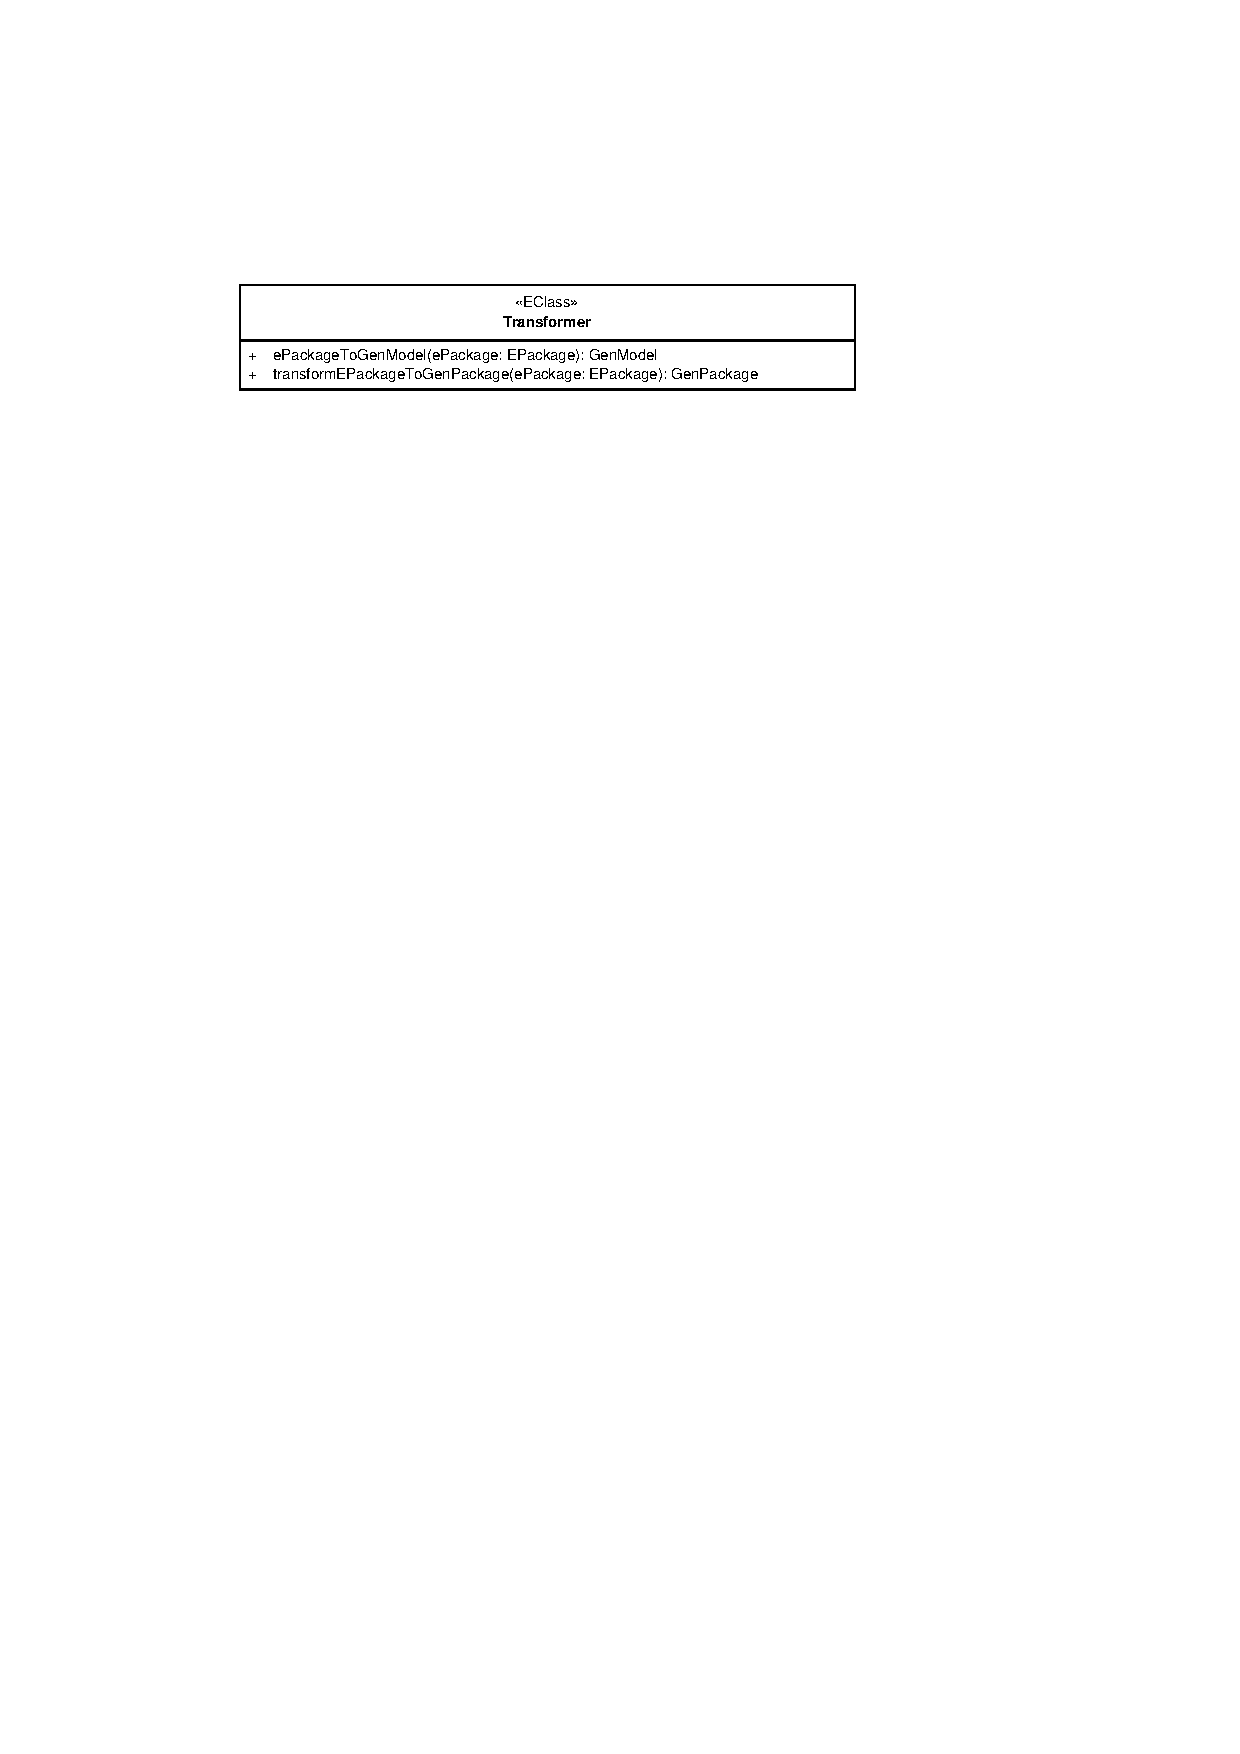
\includegraphics[width=0.7\textwidth]{../../org.moflon.doc.handbook.05_miscellaneous/3_existingEMF/emfImages/CDTransformer.pdf}
	\caption{Methods in \texttt{Transformer}}  
	\label{fig_e2gm}
	\end{center}
\end{figure} 

\vspace{1cm}

\begin{figure}[htbp]
\begin{center}  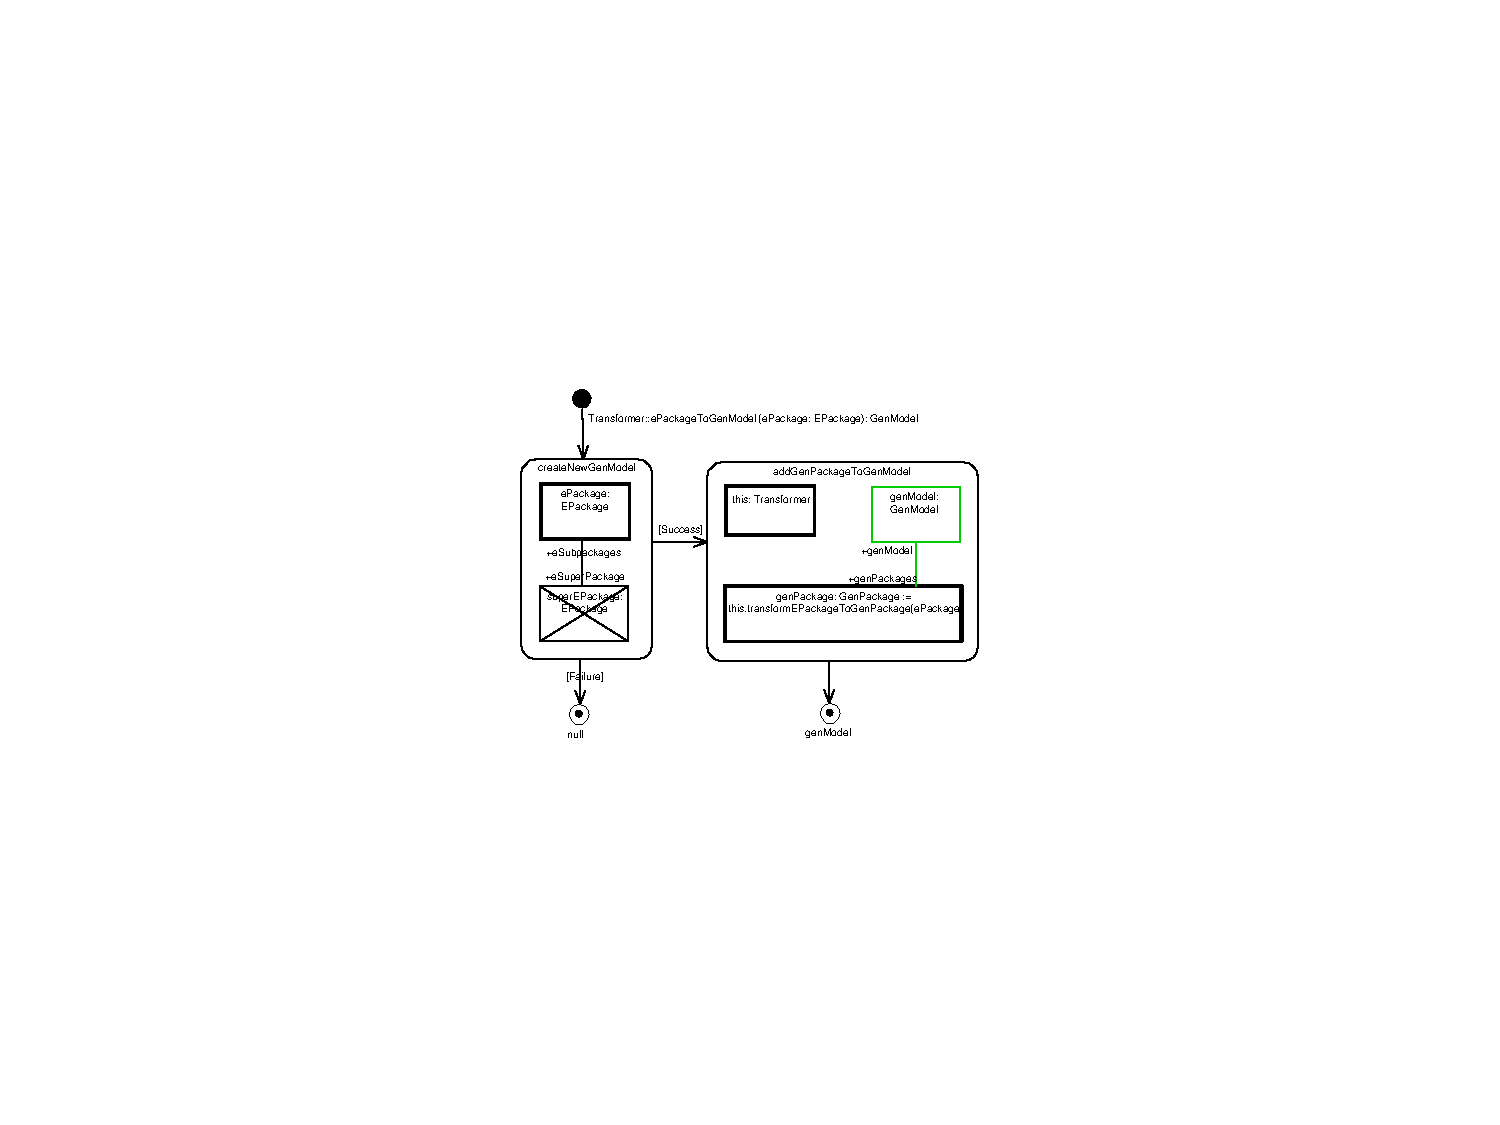
\includegraphics[width=0.8\textwidth]{../../org.moflon.doc.handbook.05_miscellaneous/3_existingEMF/emfImages/SDMePackageToGenModel.pdf}
        \caption{Main method for \texttt{EPackage} to \texttt{GenModel} transformation}  
  \label{fig_pack2g}
\end{center}
\end{figure} 

\begin{figure}[htbp]
\begin{center}  
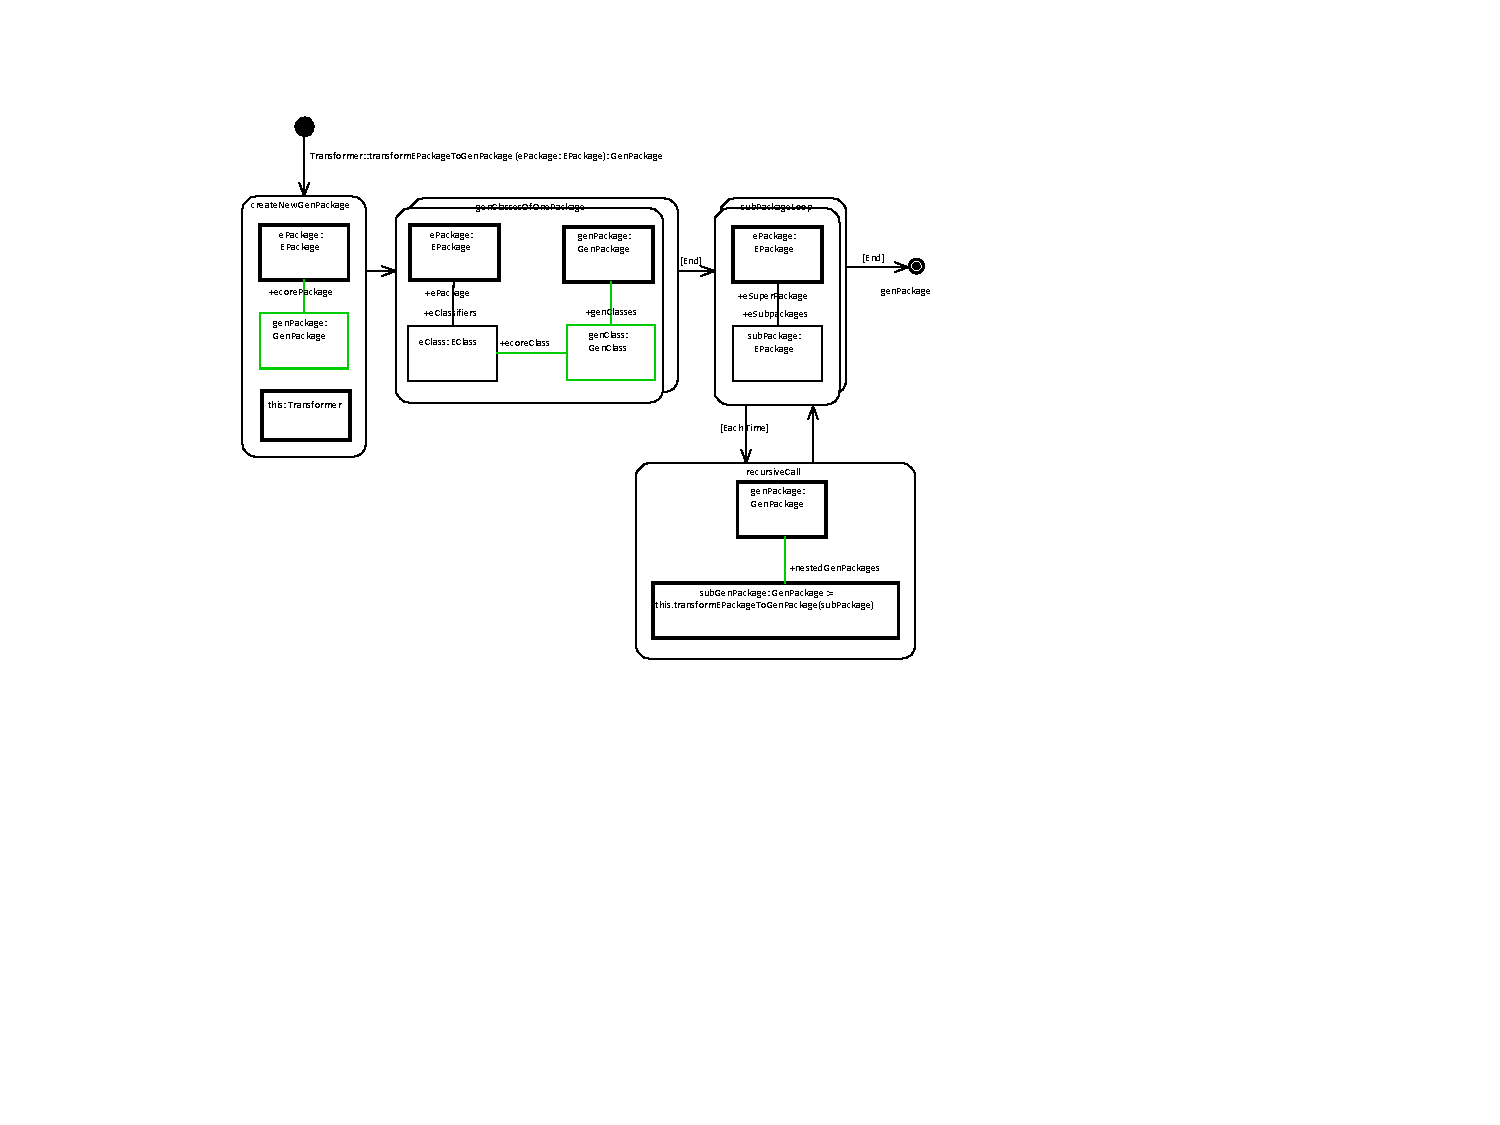
\includegraphics[width=1.1\textwidth]{../../org.moflon.doc.handbook.05_miscellaneous/3_existingEMF/emfImages/SDMtransformEpackageToGenPackage.pdf}
\caption{Helper function to transform all \texttt{EPackages} to \texttt{GenPackages}}  
\label{fig_transf}
\end{center}
\end{figure} 

